%!TEX root = <../index.tex>

\section{Experimental Results and Discussion}
\label{sec:5}

The experimental results are described, analyzed and concluded in this section. In section \ref{sec:5.1} the statistics of the corpus after preprocessing is showed briefly. Section \ref{sec:5.2} focuses on the effectiveness of the different STS models, i.e. how precise the STS models predicts an articles as related for a given target article. Furthermore, the operational performance of the STS models is reported in section \ref{sec:5.3}. The above three parts concentrate on the first experiment, which is mentioned in section \ref{sec:4.4}. On the next step, the results of the second experiment are reported in section \ref{sec:5.4}. After reporting the results of the both experiments, we discuss the most severe types of errors that an articles which is virtually unrelated is predicted as related for a target article or a cluster of articles which are properly related are never or rarely predicted as related. In conclusion, we summarize the consequence of selection of the STS models and the challenge of the current work. 

\subsection{Analysis of Preprocessing}
\label{sec:5.1}

Each article contains three semantic components including \ititle{}, \ititle{}, \isummary{} which are as input data of the framework. These components are also called data sources. After preprocessing the data sources in raw string format is converted to a sequence of phrases which consist of $n$ tokens. For the n-gram model with different value of $n = 1, 2, 3$, we have three different representation forms for every data source. A vocabulary is generated from all converted by preprocessing methods data for each representation form of each data source.

\begin{figure}[!htb]
    \centering
    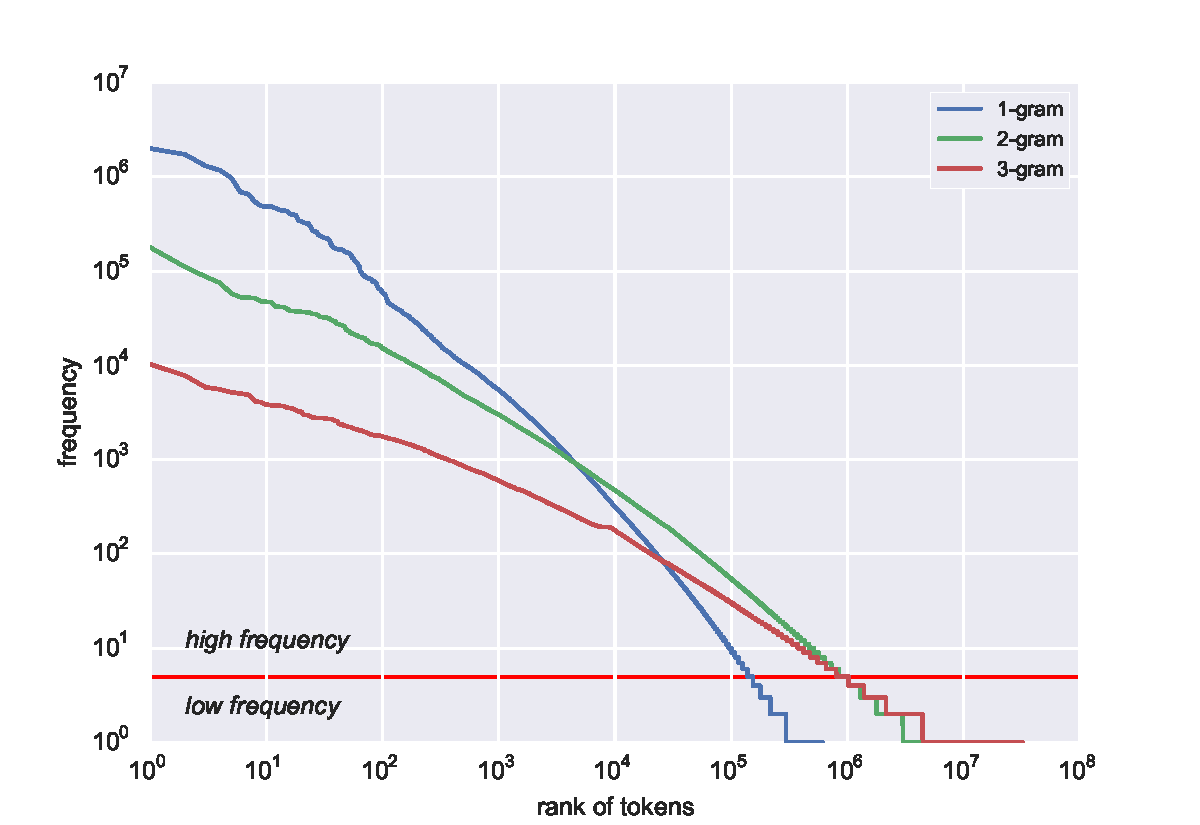
\includegraphics[width=0.8\textwidth]{fig/freqdist}
    \caption{Occurrence Frequency of terms in the corpus for uni-, bi- and trigram in descend ranking. The corresponding preprocessing is \iSE{} and the data source is \icontent{}.}
    \label{fig:freqdist}
\end{figure}

There are two main metrics to portray a vocabulary. The first metric is the size, which impacts the complexity of computing in next phases of discovering related articles. The second one is the scale of long tail of the vocabulary. According to the Zipf's law, the occurrence frequency is distributed extremely unevenly or that is to say that the most terms occur rarely in use and hence it is almost incapable to determine the semantic relevance of these terms by statistical methods. In ideal case, a vocabulary with smaller size and fewer not common used terms has the better quality with both of operational complexity and semantic completeness. Figure \ref{fig:freqdist}, which depicts a representative sample the distribution of the occurrence frequency, indicates that only a small quantity of tokens occur repetitively in the corpus (25\% for unigram, 10\% for bigram and 3\% for trigram). Taking into account efficiency, the tokens which appear less than $5$ times can be removed from the vocabulary. We denote the original vocabularies as \ifull{} vocabularies and the reduced vocabularies as \icommon{} vocabularies. 

\begin{figure}[!htb]
    \centering
    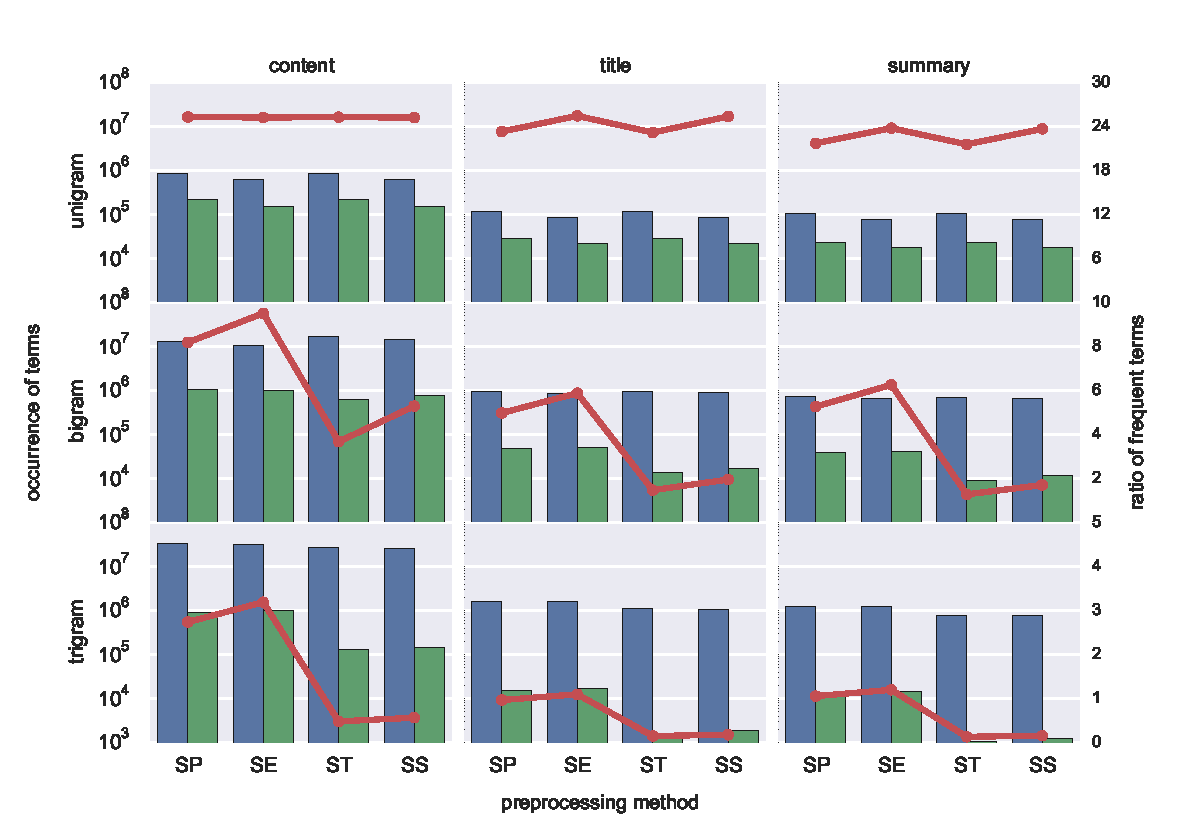
\includegraphics[width=\textwidth]{fig/vocab_size}
    \caption{Comparison the vocabulary size of different preprocessing methods for given data sources with n-gram models. Each column refers to a kind of data source, which is \icontent{}, \ititle{} and \isummary{} respectively while each row refers to a n-gram model: uni-, bi-, and trigram. \textit{Full} vocabularies are illustrated as blue bars and \icommon{} vocabularies as green bars. The red line shows the ratio of the size of \icommon{} vocabularies to the corresponding \ifull{} vocabularies. }
    \label{fig:vocab_size}
\end{figure}


We consider the size of \ifull{} vocabularies and the proportion of frequent tokens as the metrics to evaluate the vocabulary quality. Figure \ref{fig:vocab_size} shows the comparison between the size of \ifull{} and \icommon{} vocabularies which are generated by the preprocessing methods including \iSP{}, \iSE{}, \iST{} and \iSS{} in the different n-gram models ($n=1, 2, 3$) of the three kinds of data source containing \icontent{}, \ititle{} and \isummary{}. In the unigram model, \iSS{} always generates the both smallest vocabularies with the largest proportion of frequent terms. In bi- and trigram, the vocabularies generated by \iSE{} has the largest proportion of frequent terms and the size is slightly different with the vocabularies generated by other methods. In conclusion, the preprocessing method \iSS{} is applied in unigram and \iSE{} is applied in both of bigram and trigram. 


\subsection{Effectiveness of STS Models}
\label{sec:5.2}

As described in section \ref{sec:3.3}, the effectiveness metrics include \textit{precision@k@h} to evaluate the relatedness of the articles of top ranking and \textit{nDCG} to evaluate the overall results. First, the results for each data source with n-gram are given and the best STS models is selected respectively. We give a reasonable assumption that an article is related to the articles which are not farther than $3$ hops. In order to analyze the effectiveness, the assumption is relaxed or that is to say, that the effectiveness is evaluated in the cases of $1$-hop, $3$-hops, $5$-hops and $10$-hops. In the end of the section, the divergence between different categories is discussed and which categories the framework is more suitable for are concluded.  

\subsubsection{Parameter Selection for Topic Models}

Topic models, such as LSI and LDA, represent documents as vectors in topic space. The dimension of the topic space, as well as the number of topics is pre-defined. Hence, it is necessary to determine the optimal number of topics before building and evaluating models. Figure \ref{fig:precision_topics} shows the change in precision and operational time of LSI with increasing the number of topics from $50$ to $1000$. The precision keeps increasing but the growth becomes weaker and weaker, when the number of topics becomes larger. On the other side, the time cost of both of building and predicting increases with a relative stable growth speed. We selects $500$ as the final value of this hyperparameter, because the precision increases quite insignificantly with more than $500$ topics and we expect that the building time is limited to less than one hour and the predicting time is limited to less than one second. 

\begin{figure}[!htb]
    \centering
    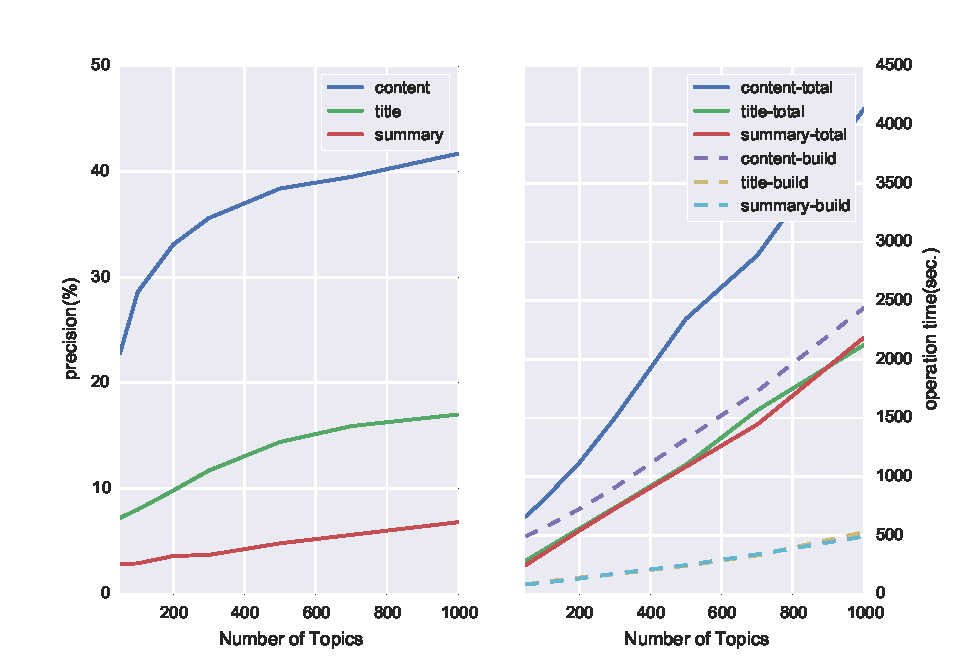
\includegraphics[width=\textwidth]{fig/precision_topics}
    \caption{Precision@2@3 and the time cost of LSI with the different value of the number of topics. Models are built with the historical corpus of $73908$ articles and predict related articles for $2000$ randomly selected articles. The dash line indicates the building time and the solid line indicates the total time including building and predicting. }
    \label{fig:precision_topics}
\end{figure}


\subsubsection{Overall Analysis of Effectiveness}

The five STS models are applied for the nine separated semantic data ( (\icontent{}, \ititle{}, \isummary{}) $\times$ (unigram, bigram, trigram)). We apply \textit{precision@2@3} and \textit{nDCG} for evaluating the effectiveness of the models. 

Figure \ref{fig:precision_2_3} compares the precision of the STS models in the different data. In general, the models perform in \icontent{} better than in \ititle{} and much better than in \isummary{}. Second, the precision in unigram is better than in bigram and the precision in trigram is the worst. To be specific, \textit{tfidf} preforms the highest precision for all data sources in unigram and for \icontent{} and \ititle{} in bigram. In the meanwhile, \textit{Jaccard} is stronger than the other models for \isummary{} in bigram and all data sources in trigram. \textit{LDA} is the weakest model all the time in the experiment and it is skipped in bigram and trigram to avoid unnecessary costs. The precision of \textit{BoW} is slightly ($10\% \sim 30\%$) lower than the best model and, however, it is $30\% \sim 60\%$ lower than the best model in bigram and trigram. 


\begin{figure}[!htb]
    \centering
    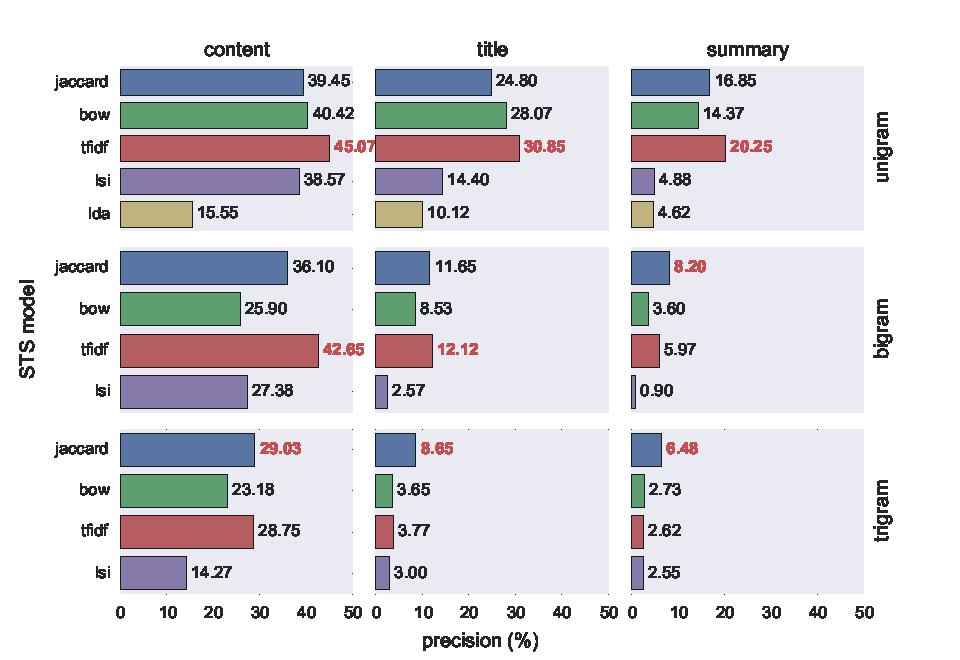
\includegraphics[width=\textwidth]{fig/precision_2_3}
    \caption{comparison the precision of \textit{jaccard}, \textit{BoW}, \textit{tfidf}, \textit{LSI} and \textit{LDA} for all data sources  with n-gram models. }
    \label{fig:precision_2_3}
\end{figure}

Figure \ref{fig:ndcg} illustrates the \textit{nDCG}, which is applied as the supplementary evaluation method. The order of models by \textit{nDCG} is similar to the results of \textit{precision} in general. All STS models are capable to discover related articles, because the measure \textit{nDCG} of every model is better than the baseline, which is computed for the random order of candidates. Moreover, LSI performs better in the metric \textit{nDCG} than in the metric \textit{precision} for the data source \icontent{}. To be specific, LSI is almost always at the second position after tfidf in \textit{nDCG}, whereas LSI is at the third or the last position in \textit{precision}. Accordingly, LSI computes the more precise relatedness of the overall corpus than jaccard and BoW, while LSI is not able to determine precisely which articles have the highest relatedness. 


\begin{figure}[!htb]
    \centering
    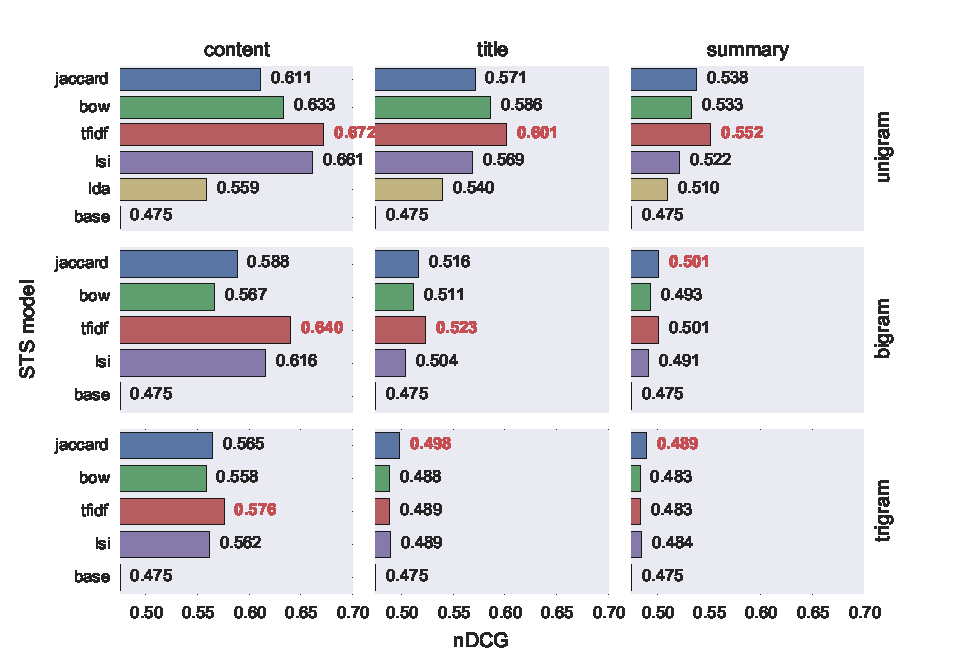
\includegraphics[width=\textwidth]{fig/ndcg}
    \caption{comparison the nDCG of jaccard, BoW, tfidf, LSI and LDA for all data sources with n-gram models.}
    \label{fig:ndcg}
\end{figure}


Combining the results of two evaluation methods, we conclude as follows.

1. Relatedness generated from data source \ititle{} or \isummary{} is worse than from \icontent{}, because \ititle{} and \isummary{} are short documents and then contain incomplete information. 

2. In n-gram, the vocabulary becomes larger and the relevance between phrases become weaker along with a greater $n$. On the other hand, a higher $n$ leads to the more serious loss of semantic information with removing the low frequency terms from the vocabulary. A typical example is that $77\%$ information/phrases are dropped through reducing vocabulary for \icontent{} in trigram. 

3. Tfidf is in the dominant position for uni-/bigram and long documents and jaccard is more suitable in trigram and short documents. Unexpected, LDA works with unsatisfactory effectiveness. 


%\subsubsection{Coverage of Related Articles Prediction}

\begin{table}[!htb]
\centering
\resizebox{\textwidth}{!}{%
\begin{tabular}{lrr|rr|rr|rr|rr|rr|rr|rr|rr}
 & \multicolumn{6}{c|}{\textbf{Content}} & \multicolumn{6}{c|}{\textbf{Title}} & \multicolumn{6}{c}{\textbf{Summary}} \\
 & \multicolumn{2}{c|}{\textbf{1-tfidf}} & \multicolumn{2}{c|}{\textbf{2-tfidf}} & \multicolumn{2}{c|}{\textbf{3-jaccard}} & \multicolumn{2}{c|}{\textbf{1-tfidf}} & \multicolumn{2}{c|}{\textbf{2-tfidf}} & \multicolumn{2}{c|}{\textbf{3-jaccard}} & \multicolumn{2}{c|}{\textbf{1-tfidf}} & \multicolumn{2}{c|}{\textbf{2-jaccard}} & \multicolumn{2}{c}{\textbf{3-jaccard}} \\
 & \multicolumn{1}{c}{\textbf{r}} & \multicolumn{1}{c|}{\textbf{diff}} & \multicolumn{1}{c}{\textbf{r}} & \multicolumn{1}{c|}{\textbf{diff}} & \multicolumn{1}{c}{\textbf{r}} & \multicolumn{1}{c|}{\textbf{diff}} & \multicolumn{1}{c}{\textbf{r}} & \multicolumn{1}{c|}{\textbf{diff}} & \multicolumn{1}{c}{\textbf{r}} & \multicolumn{1}{c|}{\textbf{diff}} & \multicolumn{1}{c}{\textbf{r}} & \multicolumn{1}{c|}{\textbf{diff}} & \multicolumn{1}{c}{\textbf{r}} & \multicolumn{1}{c|}{\textbf{diff}} & \multicolumn{1}{c}{\textbf{r}} & \multicolumn{1}{c|}{\textbf{diff}} & \multicolumn{1}{c}{\textbf{r}} & \multicolumn{1}{c}{\textbf{diff}} \\ \hline
\textbf{Mean} & \multicolumn{2}{c|}{45.07} & \multicolumn{2}{c|}{42.65} & \multicolumn{2}{c|}{29.03} & \multicolumn{2}{c|}{30.85} & \multicolumn{2}{c|}{12.12} & \multicolumn{2}{c|}{8.65} & \multicolumn{2}{c|}{20.25} & \multicolumn{2}{c|}{8.20} & \multicolumn{2}{c}{6.48} \\ \hline
\textbf{\textcolor{blue}{Gesellschaft}} & 3 & $+~~8.75$ & 4 & $+~~6.89$ & 2 & $+17.38$ & 3 & $+15.20$ & 4 & $+13.20$ & 2 & $+53.01$ & 2 & $+14.98$ & 2 & $+28.53$ & 2 & $+43.84$ \\
\textbf{\textcolor{blue}{Politik}} & 4 & $+~~8.24$ & 1 & $+14.57$ & 1 & $+41.88$ & 4 & $+~~6.97$ & 6 & $+~~5.00$ & 5 & $+~~6.89$ & 1 & $+16.26$ & 3 & $+16.23$ & 3 & $+10.94$ \\
\textbf{Digital} & 1 & $+15.83$ & 2 & $+~~9.97$ & 7 & $-34.45$ & 1 & $+24.78$ & 5 & $+13.13$ & 7 & $-23.27$ & 3 & $+~~9.25$ & 6 & $-19.06$ & 8 & $-31.66$ \\
\textbf{Kultur} & 6 & $-~~5.28$ & 6 & $-~~9.53$ & 9 & $-52.02$ & 6 & $-~~3.05$ & 1 & $+44.99$ & 4 & $+~~8.22$ & 4 & $+~~3.73$ & 4 & $+14.16$ & 5 & $+~~5.78$ \\
\textbf{Lebensart} & 10 & $-34.97$ & 10 & $-35.32$ & 6 & $-28.72$ & 9 & $-27.35$ & 2 & $+42.20$ & 1 & $+59.46$ & 9 & $-31.89$ & 1 & $+47.18$ & 1 & $+59.77$ \\
\textbf{Sport} & 7 & $-~~7.26$ & 5 & $-~~8.71$ & 5 & $-18.10$ & 7 & $-16.31$ & 3 & $+35.20$ & 8 & $-24.19$ & 5 & $-~~8.93$ & 5 & $-~~5.04$ & 6 & $-~~5.06$ \\
\textbf{Wissen} & 2 & $+13.10$ & 3 & $+~~8.04$ & 4 & $-17.81$ & 2 & $+15.46$ & 9 & $-38.01$ & 9 & $-24.44$ & 7 & $-14.47$ & 9 & $-32.25$ & 10 & $-44.48$ \\
\textbf{Karriere} & 5 & $+~~6.58$ & 7 & $-12.65$ & 8 & $-42.58$ & 5 & $-~~1.48$ & 10 & $-43.40$ & 6 & $-20.66$ & 6 & $-12.85$ & 8 & $-28.26$ & 4 & $+~~5.99$ \\
\textbf{\textcolor{red}{Wirtschaft}} & 8 & $-14.73$ & 8 & $-17.52$ & 3 & $-13.03$ & 8 & $-19.23$ & 8 & $-36.87$ & 10 & $-26.57$ & 8 & $-15.55$ & 7 & $-20.55$ & 7 & $-11.96$ \\
\textbf{\textcolor{red}{Reisen}} & 9 & $-30.22$ & 9 & $-31.93$ & 10 & $-52.77$ & 10 & $-34.65$ & 7 & $-20.19$ & 3 & $+11.88$ & 10 & $-64.16$ & 10 & $-50.83$ & 9 & $-37.73$ \\
\textbf{\textcolor{red}{Studium}} & 11 & $-61.03$ & 11 & $-49.30$ & 11 & $-67.41$ & 11 & $-43.05$ & 11 & $-66.56$ & 11 & $-37.51$ & 11 & $-73.31$ & 11 & $-83.52$ & 11 & $-79.13$ \\ \hline
\end{tabular}%
}
\caption{Comparison between the precision of different categories and the mean precision of the entire corpus. \textbf{r} refers to the ranking of precision in all categories and \textbf{diff} indicates the ratio (\%) of difference compared with the mean precision ($diff = \frac{prec_{cate} - prec_{mean}}{prec_{mean}}\times 100\%$)}
\label{tab:cate_precision}
\end{table}

\subsubsection{Divergence between Categories}

The effectiveness is reported and analyzed above in general. Now we are also interested, how the models, which are selected as the best models for each data set respectively, work for specific categories. The results are drawn in table \ref{tab:cate_precision}, where the precision ranking of each category and the difference ratio to the mean precision of the entire corpus are revealed. \textit{Gesellschaft} (\textit{society}) and \textit{Politik} (\textit{politics}) surpass the mean precision in all data set. On the contrary, \textit{Wirtschaft} (\textit{economics}), \textit{Reisen} (\textit{traval}) and \textit{Studium} (\textit{study}) are the worst performed categories. The precision of these three categories is much lower than the mean level. Taking content-unigram as example, the precision of the best category (\textit{Digital}) is about three times greater than the precision of the weakest category (\textit{Studium}). The results of predicting hence have  different confidence according to the category which the target article belongs to. Once the confidence of particular categories is lower than the threshold, the framework is not suitable for theses categories. 

\subsection{Efficiency of STS Models}
\label{sec:5.3}

The complete workflow of the framework can be simplified to two main phases, scilicet building phase and predicting phase. In building phase, the historical corpus is utilized and transformed through the sub-phases successively including preprocessing, vocabulary generating, model training/building and transforming. After building phase, articles from the historical corpus are represented as vectors or term-set, by the model. Then, predicting phase is the phase to discover related articles for target articles through vector representing, \textit{cosine} similarity computing and whereby ordering. 

The time cost of preprocessing is not taken into account, since the cost is tiny and more importantly preprocessing does not depend on the selection of STS models nor n-gram models. In following we analyse efficiency on three views: internal comparison between STS models, vertical comparison between n-gram models, and horizontal comparison between data sources. 

\subsubsection{Comparison of building time}

The results of building time from experiment 1 are illustrated in figure \ref{fig:build_time} and analyzed as follows. 

\begin{figure}[!htb]
    \centering
    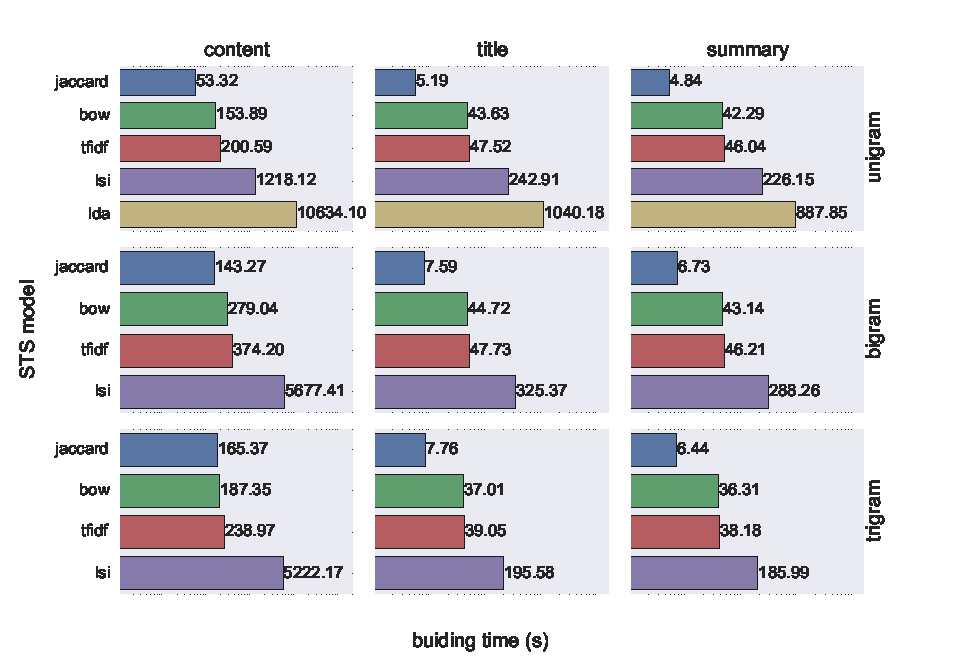
\includegraphics[width=\textwidth]{fig/building_time}
    \caption{Time cost of building phase}
    \label{fig:build_time}
\end{figure}

\begin{itemize}


\item Building phase of jaccard spends less time than other VSMs. Unlike VSMs, there is no model as ``middleware'' between articles and representation for jaccard. The building phase of jaccard is actually the phase where one article is reduced as a set of appeared terms. 

\item The building time cost of BoW and tdidf is roughly the same and tfidf spends slightly more time than BoW, because tdidf extends BoW with computing tf-idf weight. 

\item Topic models are more expensive. To be specific, LSI consumes more than 5 times for \icontent{} in unigram and even more than 20 times as much as the time tfidf consumes because of computing SVD. More seriously, the building time of LDA is 47 times as high as the building time of tfidf for \icontent{} in unigram and the time cost exceeds an acceptable range in bi- and trigram. 

\item Compared with unigram, the building time cost of jaccard, BoW, tfidf, LSI for \icontent{} in bigram, is increased by 3.2 times, 2.1 times, 2.1 times and 4.6 times, respectively, where as the time cost increases by only 2.4 times, 1.2 times, 1.2 times and 4.2 times correspondingly. On the other hand, the time cost of a particular STS model is not significantly different between uni-, bi- and trigram.

\end{itemize}

\subsubsection{Comparison of predicting time}

The results of predicting time are illustrated in figure \ref{fig:predict_time} and analyzed as follows. 
\begin{figure}[!htb]
    \centering
    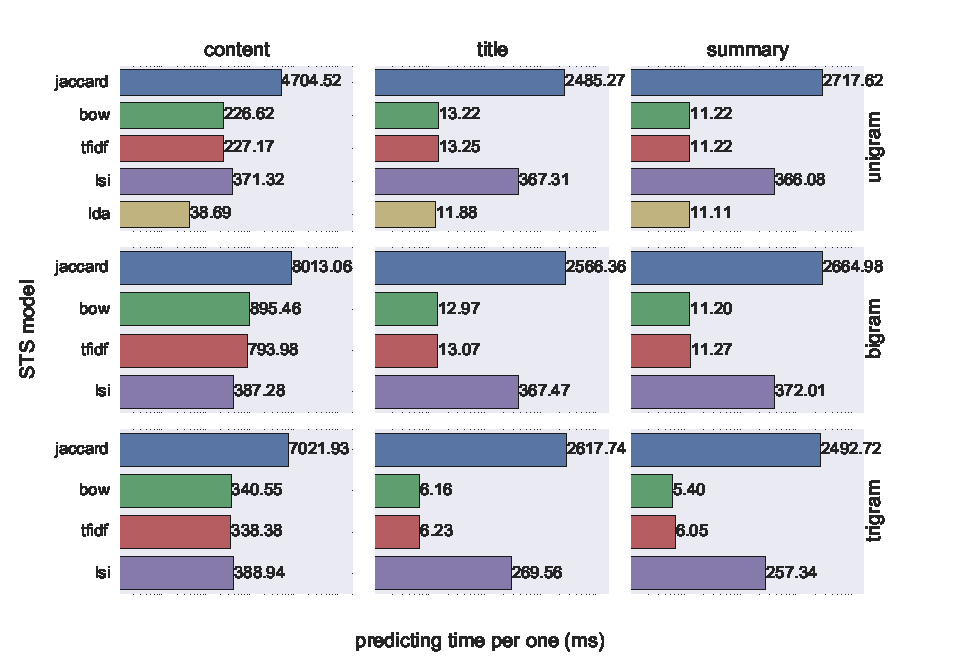
\includegraphics[width=\textwidth]{fig/predicting_time}
    \caption{Time cost of predicting related articles for one target}
    \label{fig:predict_time}
\end{figure}

\begin{itemize}
\item Similar to building phase, jaccard is also quite different from other VSMs. The jaccard similarity between two documents is computed by dividing the size of union of the corresponding term sets by the size of intersection of them. This operation is more costly than computing \textit{cosine} similarity between vectors. As compared with tfidf, jaccard costs 20-fold, 10-fold and 21 fold time for \icontent{} in uni-, bi- and trigram, respectively.

\item Predicting phase consists of representing phase and similarity computing phase. The first phase depends on the complexity of the corresponding model. Specifically, a document is represented as a vector of occurrence frequency, tf-idf weight and topic weight for BoW, tfidf and topic modles(i.e. LSI and LDA), respectively, and complexity increases progressively. The second phase depends on the vector dimension and the amount of vectors. Normally, the vector dimension of topic models is much lower than BoW and tfidf and hence, topic models cost less time in the second phase. In \icontent{}, the cost of LSI is similar to BoW and tfidf, whereas it is much higher than BoW and tfidf in \ititle{} and \isummary{}, which generate much smaller vocabularies and accordingly the lower vector dimension. 

\end{itemize} 

In conclusion, we determine the final selection of the best model for each dataset in table \ref{tab:select}, taking into account both of effectiveness and efficiency.

\begin{table}[!htb]
\centering
\begin{tabular}{|c|c|c|c|}
\hline
\textbf{Model} & \textbf{Content} & \textbf{Title} & \textbf{Summary} \\ \hline
\textbf{Unigram} & tfidf & tfidf & tfidf \\ \hline
\textbf{Bigram} & tfidf & tfidf & jaccard \\ \hline
\textbf{Trigram} & tfidf & jaccard & jaccard \\ \hline
\end{tabular}
\caption{Model selection for each data source in n-gram.}
\label{tab:select}
\end{table}

\subsection{Results of Incremental Updating}
\label{sec:5.4}

\subsubsection{Effectiveness}

\subsubsection{Efficiency}

\subsection{Error Analysis}
\label{sec:5.5}

We present insights on the most severe types of errors of false positive and false negative that occurred in the experiments. In order to confirm the reasons or conditions of the errors, we inspect manually the predictions of the framework to discover related articles and compare them with the golden standard understanding of human beings.  

\subsubsection{False Positive Error}

A false positive error is a result that indicates a given condition has been fulfilled, when it actually has not been fulfilled. In our case, a false positive error is the event that an article which is actually unrelated to the target article is assigned as related by the framework. 

\begin{itemize}
    \item One type of fp errors is caused by the labeled corpus we select. The list of related articles is marked by the editor manually and the size is limited up to $2$. Therefore, the list is incomplete, so that articles which should be related to each other under human understanding are unreachable to each other in the related-graph generated based on the lists of related articles. Only this type is not the real errors but the inherent systematic lack. 
    
    Example: 
    \begin{itemize}
        \item \textit{``Tod dem Diktator'' - Rufe zur Vereidigung} (\textit{``Death to the dictator'' - require for swearing}) \footnote{\url{http://www.zeit.de/online/2009/32/iran-proteste-vereidigung/komplettansicht}}
        \item \textit{Proteste in Teheran dauern an} (\textit{Protests in Tehran persist}) \footnote{\url{http://www.zeit.de/online/2009/32/iran-ahmadineschad-proteste/komplettansicht}}
    \end{itemize}
    The both articles report the protest against Mahmoud Ahmadinejad, who is re-elected as the Iranian president, and the international as well as authoritative reaction. The articles should be related by the human judgement, but there is no related-path between them. We consider that the incompleteness of labeling causes the fp error. 
    
    \item One article usually contains a set of topics rather than the single topic. The topics are not treated equally, but they are understood in different importance. It is complicate and subtle, how human beings weigh the importance of different topics. Out of this view point, two articles are assigned as related, only when they share the topics with the highest weight, otherwise they are unrelated, even though they are similar to each other in semantic or lexical meaning. 
    
    Example:
    \begin{itemize}
        \item \textit{Tunesiens Innenminister wird neuer Regierungschef} (\textit{Tunisia Interior Minister appointed new head of government}) \footnote{\url{http://www.zeit.de/politik/ausland/2013-02/tunesien-regierungschef-larayedh-jebali}}
        \item \textit{Tunesien hebt den Ausnahmezustand seit Arabellion auf} (\textit{Tunisia cancels the state of emergency beginning from Arabellion}) \footnote{\url{http://www.zeit.de/politik/ausland/2014-03/tunesien-ausnahmezustand-aufhebung}}
    \end{itemize}
    
    The both articles mention the identical background, subject of the events and keywords. However, the critical reported topics are different and unrelated. In addition, quite a few named entities which they share confuse the framework predicts the relatedness between them. 
    
\end{itemize}


c. 有相似内容,但是中心主题无关,
Dem Präsidentenpaar droht eine herbe Wahlniederlage - \footnote{\url{http://www.zeit.de/online/2009/27/argentinien-wahl-kirchner}}
Der Schattenpräsident - \footnote{\url{http://www.zeit.de/politik/ausland/2010-10/nestor-kirchner-nachruf/komplettansicht}}

d. 无相关内容,完全错误预测
Ohne Gras kein Spaß - \footnote{\url{http://www.zeit.de/2009/20/Portugal-Golf/komplettansicht}}
Jonglieren entspannt und macht schlau - \footnote{\url{http://www.zeit.de/karriere/beruf/2012-10/konzentration-gehirnleistung-jonglage/komplettansicht}}

2. examples for false negative
a. 介绍宏观问题和报道具体例子
Uni Leipzig droht mit Schließung ganzer Fakultäten - \footnote{\url{http://www.zeit.de/studium/hochschule/2014-02/universitaet-leipzig-finanzierung}}
Drittmittel sind ungleich verteilt - \footnote{\url{http://www.zeit.de/studium/hochschule/2014-02/Drittmittel-an-Hochschulen}}

b. 讨论同一主题下的不同分支内容
Der Jugendschutzfilter blockiert zu viel - \footnote{\url{http://www.zeit.de/digital/internet/2012-02/jugendschutzfilter-filtern-blogs/komplettansicht}}
Filmwirtschaft weitet Selbstkontrolle auf Internet aus - \footnote{\url{http://www.zeit.de/kultur/film/2011-10/fsk-jugendschutz-internet}}

c. 只是基于同样的背景,而描述的事情并不相同,只是表达的情感、理念或观点相同。
"Die Koordination durch Tepco ist oft furchtbar" - \footnote{\url{http://www.zeit.de/wissen/umwelt/2014-03/interview-fukushima-drei-jahre-arbeiter/komplettansicht}}
Geächtet wie einst Japans Atombomben-Opfer - \footnote{\url{http://www.zeit.de/wissen/gesundheit/2014-03/fukushima-strahlenopfer-stigma-radioaktivitaet}}
\subsection{Conclusion}
\label{sec:5.6}
1. 分析了性能,分析了错误
2. 最好的是content-1-tfidf,其他的见表格
3. 问题是没有使用corpus中的标记,即保存的人工标记related。利用这些数据,会训练出更加specific更加precise的模型,在下一章详细说明。